% LaTeX Template for Project Report, Version 2.0
% (Abstracted from a Major Project Report at CSED, NIT Calicut but can be
% modified easily to use for other reports also.)
%
% Released under Creative Commons Attribution license (CC-BY)
% Info: http://creativecommons.org/licenses/by/3.0/
%
% Created by: Kartik Singhal
% BTech CSE Batch of 2009-13
% NIT Calicut
% Contact Info: kartiksinghal@gmail.com
%
% It is advisable to learn the basics of LaTeX before using this template.
% A good resource to start with is http://en.wikibooks.org/wiki/LaTeX/
%
% All template fields are marked with a pair of angular brackets e.g. <title here>
% except for the ones defining citation names in ref.tex.
%
% Empty space after chapter/section/subsection titles can be used to insert text.
%
% Just compile this file using pdflatex after making all required changes.

\documentclass[12pt,a4paper]{report}
\usepackage[pdftex]{graphicx} %for embedding images
\usepackage{url} %for proper url entries
\usepackage[bookmarks, colorlinks=false, pdfborder={0 0 0}, pdftitle={<pdf title here>}, pdfauthor={<author's name here>}, pdfsubject={<subject here>}, pdfkeywords={<keywords here>}]{hyperref} %for creating links in the pdf version and other additional pdf attributes, no effect on the printed document
%\usepackage[final]{pdfpages} %for embedding another pdf, remove if not required

\begin{document}
\renewcommand\bibname{References} %Renames "Bibliography" to "References" on ref page

%include other pages
\begin{titlepage}

\begin{center}

\textup{\small {\bf IT206 Course Project} \\ Report}\\[0.2in]

% Title
\Large \textbf {Chess in Java}\\[0.5in]


% Submitted by
\normalsize Submitted by \\
\begin{table}[h]
\centering
\begin{tabular}{lr}\hline \\
Roll No & Names of Students \\ \\ \hline
\\
16IT221 & Moksh Jain \\
16IT234 & Nishanth Hebbar \\
16IT222 & Anmol Jindal\\ \\ \hline 
\end{tabular}
\end{table}

\vspace{.1in}
Under the guidance of\\
{\textbf{R. Priyadarshini}}\\[0.2in]


\vfill

% Bottom of the page

\includegraphics[width=0.18\textwidth]{logo2.png}\\[0.1in]
\Large{National Institute of Technology Karnataka}\\
\normalsize
\textsc{Department of Information Technology}\\
Surathkal, Mangaluru, India -- 575 025 \\
\vspace{0.2cm}
November 2017

\end{center}

\end{titlepage}

\pagenumbering{roman} %numbering before main content starts
\tableofcontents

\newpage
\pagenumbering{arabic} %reset numbering to normal for the main content

\chapter{Synopsis}
\paragraph{}
Chess is a two-player strategy board game played on a chessboard, a checkered gameboard with 64 squares arranged in an 8×8 grid. Each player begins with 16 pieces: one king, one queen, two rooks, two knights, two bishops, and eight pawns. Each of the six piece types moves differently, with the most powerful being the queen and the least powerful the pawn. The objective is to checkmate the opponent's king by placing it under an inescapable threat of capture. We intend to implement the game of Chess in Java with a Graphical User Interface using Java Swing Library. The Java Swing Library uses Java's features such as Multithreading and Inheritance to enable flexible construction of User Interfaces.

\section{Problem Definition}
\paragraph{}
Chess is a board game involving two players.There are two sides,one using the white pieces and the other using the black pieces.Each of the sets of pieces includes:
\newline  1. One King
\newline  2. One Queen
\newline  3. Two Rooks
\newline  4. Two Bishops
\newline  5. Two Knights
\newline  6. Eight pawns

All of these pieces have their own distinct moves their own moves.
Each player plays alternately,with white always moving first.A piece cannot be moved to another square if it is already occupied,unless it is an opponent's piece in which case the opponent's piece is removed off the board.
The goal of the game is to strategize and place the opponent's king in an inescapable position and thus become the winner, while also protecting one's own king.If a conclusion cannot be reached, the game can also be declared as a draw.Given a 8*8 chessboard and the current configuration of the board as input, the code should be able to display all the possible legal moves for a selected piece.

\section{Objective}

The objective was to design a simple GUI based chess game which can be played by two users alternately,allowing them to make legal moves, utilizing the Object-Oriented Programming features of Java. During the course of the game,for a selected piece, all it's possible legal moves should be shown to the user.The game should also display when a king is under threat and when the game ends.The game should mimic the official game of chess as closely as possible.The goal was also to design a user-friendly game with a simple interface.Also the details of the players are also to be stored , including his win/loss statistics.Also the duration of the time the game can be played was also to be preset.The goal was to simulate a real chess game as closely as possible. The input to the core of the program is the 8 by 8 chessboard and the current configuration of the chess board,and the output is to present the users with all the possible legal moves for a selected piece. A visual GUI makes the input/output interaction very easy  %objective changed to problem definition
\chapter{Introduction}

The aim of the project is to implement the chess game which can be played by two users against each other.We make use of the JAVA Swing library, among other OOP features of Java to implement the project.It also provides a user-friendly environment and also the statistics of individual players can also be stored.We also time the game. Our implementation of Chess is for two players (no Artificial Intelligence). It is played on an 8x8 checkered board, with a dark square in each player’s lower left corner.

\section{Methodology}
\paragraph{}
The approach was to create class for the Game (Main Class), Player and the pieces. Since the all pieces can logically be represented by a Piece class, an abstract Piece class is created, which is further is inherited by all the pieces. This class contains some utility methods to get and set properties and an abstract method movePiece which returns possible moves, for a given piece at a given state. 

The Game class contains methods for setting up the Board, setting up the side panel, handling the clicks and maintaining the layout. The Player class contains methods for saving the Player data to a game data file and also retrieving it from the same along with some utility methods to get and set properties.

\section{System Specifications}
\paragraph{}
Java is a platform-independent language. The game only requires a Java Runtime Environment installed to function properly. The game was developed using OpenJDK 1.8.0\_144 on Ubuntu 16.04. %literature survey included in this
\chapter{Work Done}

\section{Work Done}

\subsection{Pieces}
\paragraph{}
The pieces extensively use the concept of inheritance and Abstraction. There is a an abstract Piece class which is inherited by all the 6 pieces: Pawn, Rook, Knight, Bishop, Queen and King. This abstract Piece class has an abstract method \textit{movePieces}. This method returns the possible destinations for the piece from a given position for a given board state.

\begin{figure}[htb]
\centering
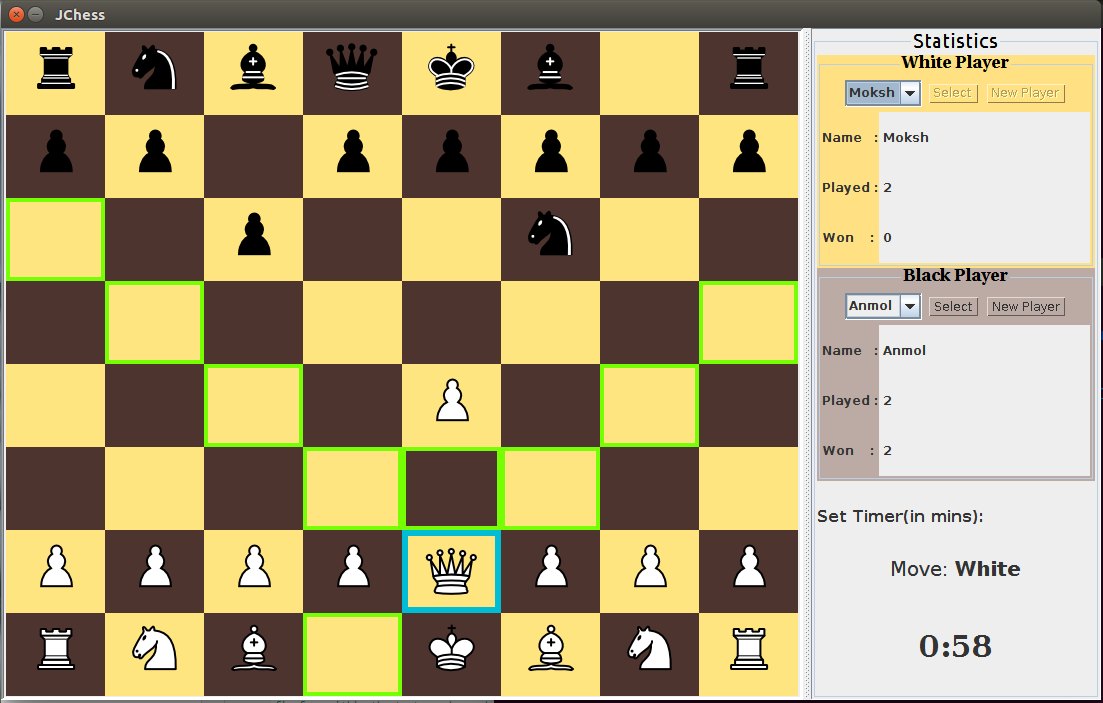
\includegraphics[scale=0.3]{SS-PossibleMoves.png} % e.g. insert ./image for image.png in the working directory, adjust scale as necessary
\caption{Possible moves being highlighted}
\label{fig:label} % insert suitable label, this is used to refer to a fig from within the text as shown above
\end{figure}

\paragraph{}
When a piece is clicked, the game obtains the possible destinations for the piece in current board configuration. These possible positions are highlighted on the board, that is, (the corresponding tiles are highlighted with a border). If the King is under check then the game filters the moves, and highlights only the moves where the king is saved from the check. If the piece is a king then the moves are filtered such that it does not move to a position where it is under a check.


\subsection{Board}
\begin{figure}[htb]
\centering
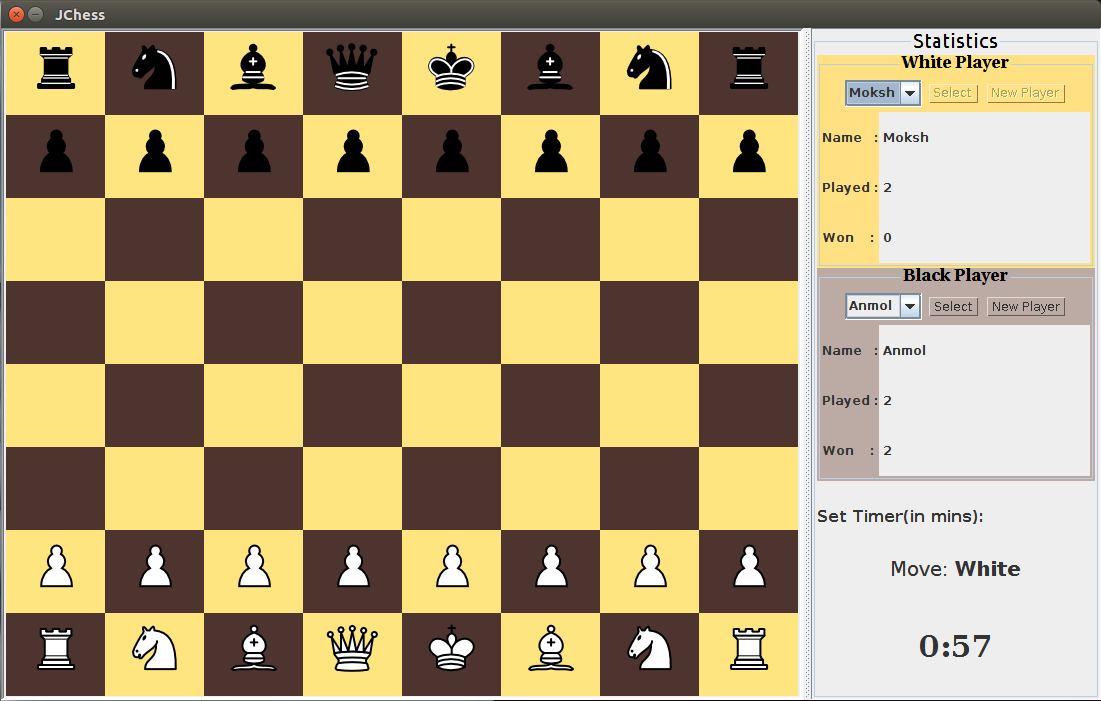
\includegraphics[scale=0.3]{SS-StartBoard.png} % e.g. insert ./image for image.png in the working directory, adjust scale as necessary
\caption{Newly created board}
\label{fig:label} % insert suitable label, this is used to refer to a fig from within the text as shown above
\end{figure}
\paragraph{}
The board consists of 64 \textit{tiles} arranged in an 8x8 grid. Each of these tiles is defined in the Tiles class. The Tile class extends extends JLabel, which is a UI Component in the Java Swing Library. Each Tile contains a reference to the piece it currently contains. The label is thus filled with the image of the corresponding piece, if any. A tile is highlighted if it is a possible destination for the current move. If the tile contains a king which is under check then it is colored red. The Tile also implements the \textit{Cloneable} Marker interface, making it easier to clone.

\subsection{Player}
\begin{figure}[htb]
\centering
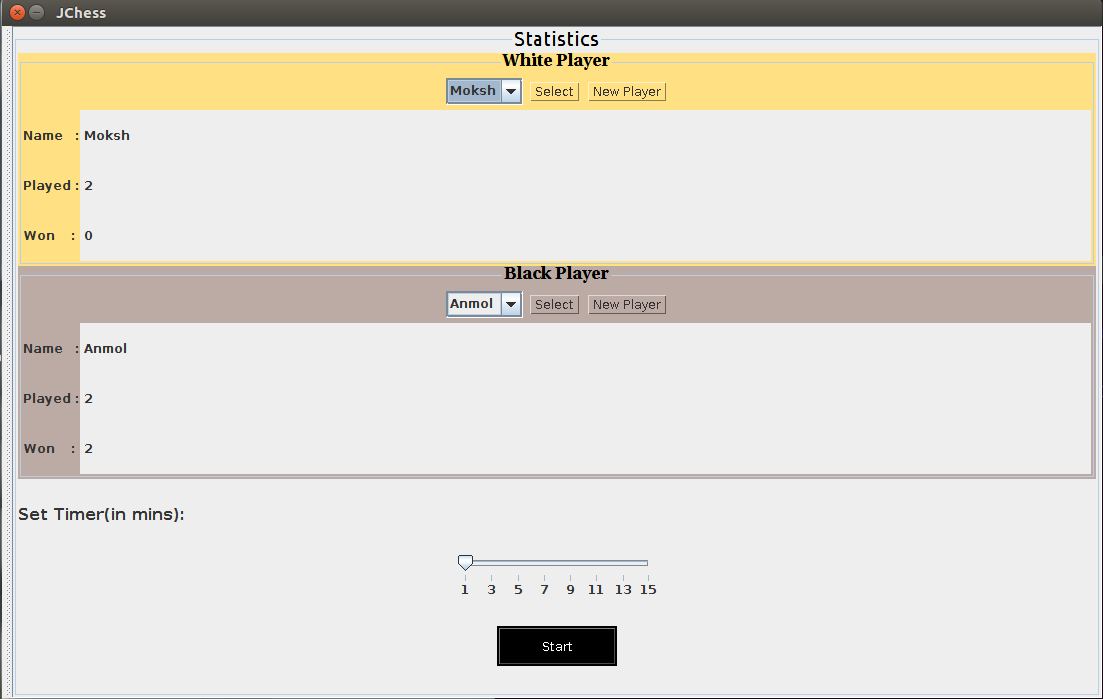
\includegraphics[scale=0.3]{SS-NewGame.png} % e.g. insert ./image for image.png in the working directory, adjust scale as necessary
\caption{User gets to select players}
\label{fig:label} % insert suitable label, this is used to refer to a fig from within the text as shown above
\end{figure}
\paragraph{}
The Player class defines the behaviour of a player in the game. It strores the name of the player, along with some other details such as games played and games won. The Player class also implements the Serializable Marker Interface to make it serializable. The Player Details are saved at the end of the game to the \textit{UserData.dat} file using the \textit{writeObject} method. When the game is started, the user can select from one of the pre-existing players stored in the game data or create a new player altogether.


\subsection{Game}
\paragraph{}
The Game class implements the main \textit{game} functionality of the the project. The Game class itself extends the JFrame class, and contains all the layouts that are displayed to the user. This includes the side panel and the board. The side panel contains the information about the Players and also displays the Timer (which can be configured at the start of the game).

\begin{figure}[htb]
\centering
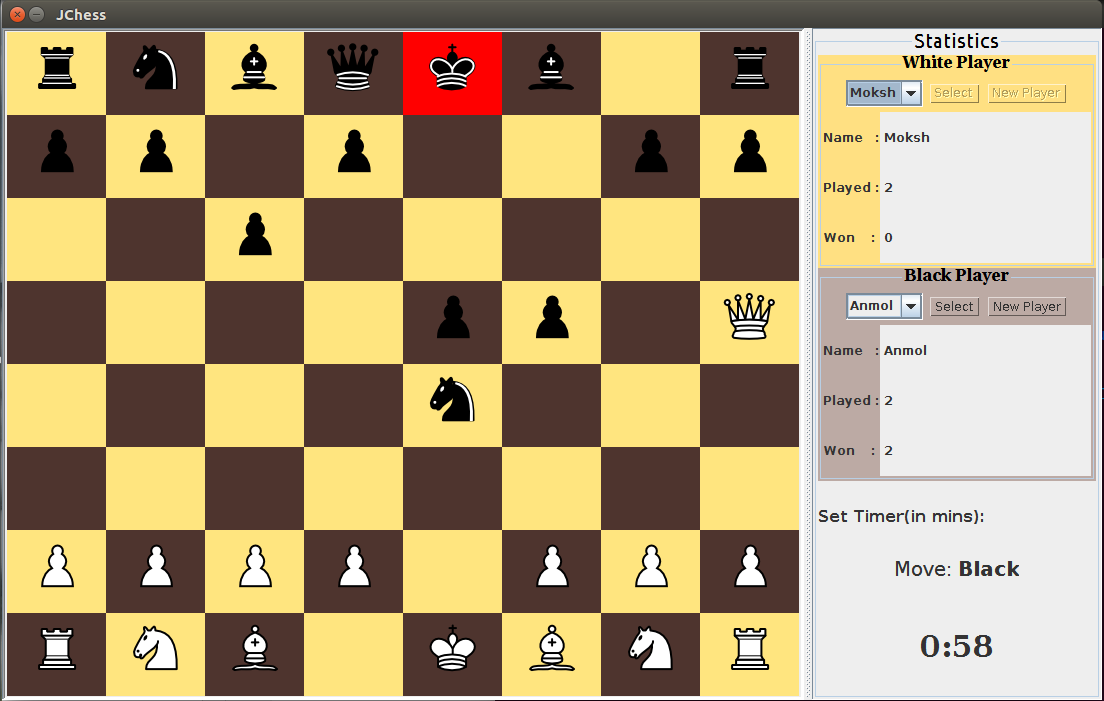
\includegraphics[scale=0.2]{SS-Check.png} % e.g. insert ./image for image.png in the working directory, adjust scale as necessary
\caption{Check}
\label{fig:label} % insert suitable label, this is used to refer to a fig from within the text as shown above
\end{figure}

\begin{figure}[htb]
\centering
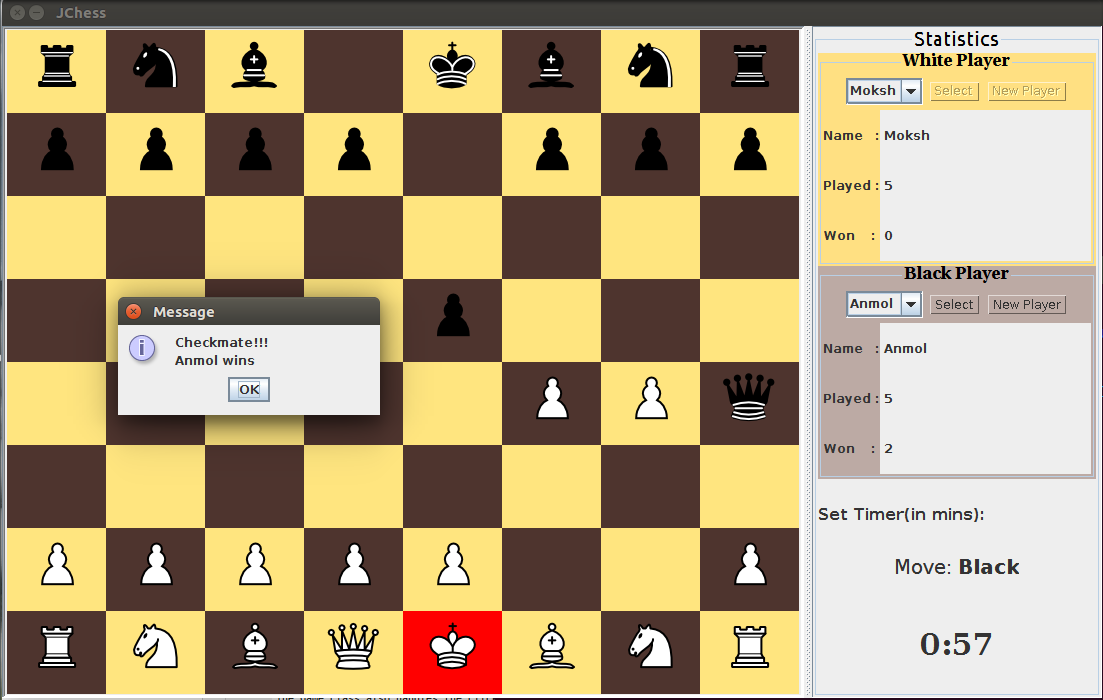
\includegraphics[scale=0.2]{SS-CheckMate.png} % e.g. insert ./image for image.png in the working directory, adjust scale as necessary
\caption{Checkmate}
\label{fig:label} % insert suitable label, this is used to refer to a fig from within the text as shown above
\end{figure}

When the game is started, the Game class is run, since it is the main class. When the game is started, the user has to select the players, and change the time limit on the timer, if required. Once the user click the \textit{Start} button, the Game class sets up the board. The Game class also handles the click event for each and appropriately highlights the possible positions and indicates if there is a check. If there is a check mate then the name of the winner is displayed and the game is restarted.

\section{Future Work}
\begin{itemize}
\item Advanced maneuvers such as castling can be implemented to make the game more function.

\item More game modes such as rapid mode can be added to make the game more versatile.

\item An AI agent can be added so the user can play against the computer in the absence of 2 players
\end{itemize}
\chapter{Conclusion}

\section{Results}
\paragraph{}
At the end, we were able to compile a \textit{.jar} file which can be run on any system with JRE available. In the project we were able to successfully implement the basic game of Chess with a GUI, using Java Swing Library. The game utilized several key concepts of object oriented programming. This includes Inheritance, Polymorphism(Runtime), Data Abstraction and Data Encapsulation. The project also utilizes features of the Java programming language to implement these concepts, such as Interfaces.

\section{Conclusion}
\paragraph{}
In the project we were able to apply the concepts of Object Oriented Programming to the implementation of the game of Chess in Java, for two players. We were also able to utilize the Java Swing GUI library which enabled us to build the Graphical User Interface for the game. The following are few of the concepts that were used among others:

\begin{itemize}
    \item Inheritance - Interfaces, Marker Interfaces, Hierarchial Inheritance
    \item Runtime Polymorphism - Method Overriding
    \item Data Abstraction - Abstract Classes and Methods
    \item Data Encapsulation - Access Modifiers
    \item GUI Design - Swing 
\end{itemize}

\section{References}
\paragraph{}
[1] Java Swing

\href{https://docs.oracle.com/javase/tutorial/uiswing/start/index.html}{https://docs.oracle.com/javase/tutorial/uiswing/start/}

\paragraph{}
[2] Java Swing Tutorials

\href{https://www.tutorialspoint.com/swing/}{https://www.tutorialspoint.com/swing/}

\paragraph{}
[3] Images of Chess Pieces.

\href{https://commons.wikimedia.org/wiki/Category:PNG_chess_pieces/Standard_transparent}{https://commons.wikimedia.org/wiki/Category:PNG\_chess\_pieces/}

\section{Appendix}

\paragraph{}
Some important snippets have been attached at the end of the report.

\paragraph{}
The full code is available at \href{https://github.com/MJ10/POP-Project}{https://github.com/MJ10/POP-Project}


\end{document}
